\section{Installation}
\subsection{Grafana}
All documetation about Grafana's installation is aviable on \href{URL}{https://grafana.com/grafana/download}.
Here the correct download for the operating system of your choice can be found, all major OSs are available : MacOS, Windows adn GNU\slash Linux and a step-by-step installation guide.
\subsubsection{Grafana WEB service}

To launch the Grafana WEB service, the following steps must be follwed dependig on which operating system is being used:

\begin{itemize}
\item\textbf{Linux}: give the following command to a in instance of a terminal:\texttt{ sudo service grafana-server start} ;
\item\textbf{Windows}: the extracted Grafana folder contains the folder "bin" with the WEB services setup file, double click on \texttt{grafana-server.exe} ;
\item\textbf{Mac}: in the "bin" folder open an instance of the  terminal and give the following comand:\texttt{ ./grafana-server web}.
\end{itemize}

Sould the user then open the preferred browser and connect to the deafult Grafana local host : \texttt{http://localhost:3000/}.
The credentials required for a first-time run are "admin" for the username field and "admin" for the password field
\begin{figure}[H]
\centering
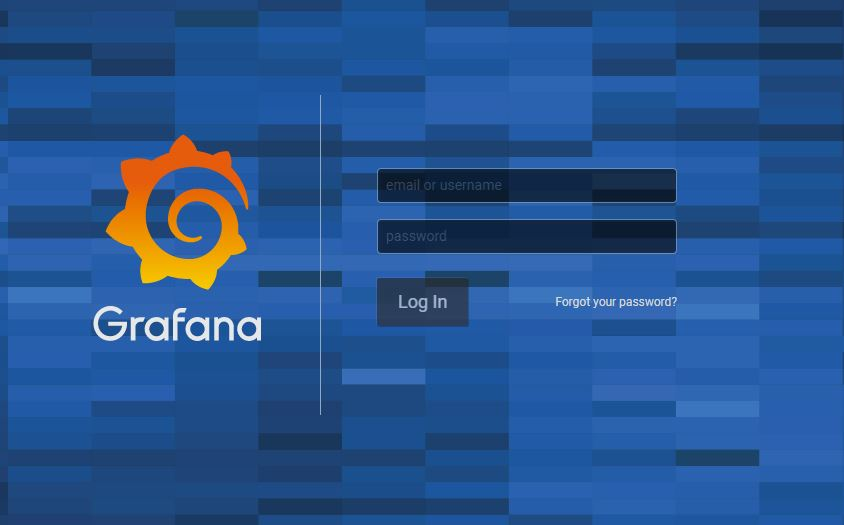
\includegraphics[scale=0.65]{img/install/login.jpg}
\caption{Grafana login page}
\end{figure}